% Created by tikzDevice version 0.12.3.2 on 2022-02-18 20:54:37
% !TEX encoding = UTF-8 Unicode
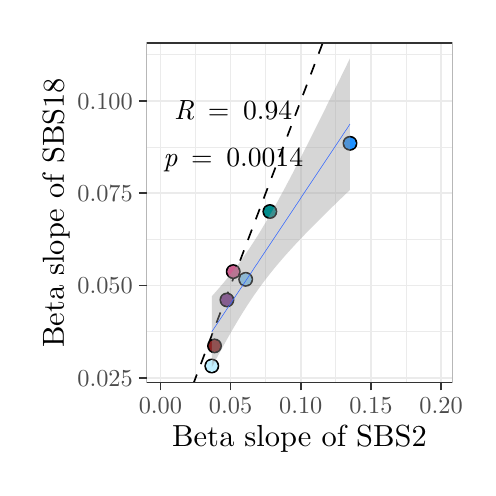
\begin{tikzpicture}[x=1pt,y=1pt]
\definecolor{fillColor}{RGB}{255,255,255}
\path[use as bounding box,fill=fillColor,fill opacity=0.00] (0,0) rectangle (158.99,158.99);
\begin{scope}
\path[clip] (  0.00,  0.00) rectangle (158.99,158.99);
\definecolor{drawColor}{RGB}{255,255,255}
\definecolor{fillColor}{RGB}{255,255,255}

\path[draw=drawColor,line width= 0.6pt,line join=round,line cap=round,fill=fillColor] (  0.00,  0.00) rectangle (158.99,158.99);
\end{scope}
\begin{scope}
\path[clip] ( 42.95, 30.69) rectangle (153.49,153.49);
\definecolor{fillColor}{RGB}{255,255,255}

\path[fill=fillColor] ( 42.95, 30.69) rectangle (153.49,153.49);
\definecolor{drawColor}{gray}{0.92}

\path[draw=drawColor,line width= 0.3pt,line join=round] ( 42.95, 49.09) --
	(153.49, 49.09);

\path[draw=drawColor,line width= 0.3pt,line join=round] ( 42.95, 82.48) --
	(153.49, 82.48);

\path[draw=drawColor,line width= 0.3pt,line join=round] ( 42.95,115.87) --
	(153.49,115.87);

\path[draw=drawColor,line width= 0.3pt,line join=round] ( 42.95,149.26) --
	(153.49,149.26);

\path[draw=drawColor,line width= 0.3pt,line join=round] ( 60.65, 30.69) --
	( 60.65,153.49);

\path[draw=drawColor,line width= 0.3pt,line join=round] ( 86.00, 30.69) --
	( 86.00,153.49);

\path[draw=drawColor,line width= 0.3pt,line join=round] (111.35, 30.69) --
	(111.35,153.49);

\path[draw=drawColor,line width= 0.3pt,line join=round] (136.70, 30.69) --
	(136.70,153.49);

\path[draw=drawColor,line width= 0.6pt,line join=round] ( 42.95, 32.40) --
	(153.49, 32.40);

\path[draw=drawColor,line width= 0.6pt,line join=round] ( 42.95, 65.79) --
	(153.49, 65.79);

\path[draw=drawColor,line width= 0.6pt,line join=round] ( 42.95, 99.18) --
	(153.49, 99.18);

\path[draw=drawColor,line width= 0.6pt,line join=round] ( 42.95,132.57) --
	(153.49,132.57);

\path[draw=drawColor,line width= 0.6pt,line join=round] ( 47.98, 30.69) --
	( 47.98,153.49);

\path[draw=drawColor,line width= 0.6pt,line join=round] ( 73.33, 30.69) --
	( 73.33,153.49);

\path[draw=drawColor,line width= 0.6pt,line join=round] ( 98.68, 30.69) --
	( 98.68,153.49);

\path[draw=drawColor,line width= 0.6pt,line join=round] (124.03, 30.69) --
	(124.03,153.49);

\path[draw=drawColor,line width= 0.6pt,line join=round] (149.37, 30.69) --
	(149.37,153.49);
\definecolor{drawColor}{RGB}{0,0,0}

\path[draw=drawColor,line width= 0.6pt,dash pattern=on 4pt off 4pt ,line join=round] ( 48.36,  0.00) -- (108.71,158.99);
\definecolor{fillColor}{RGB}{0,0,0}

\path[draw=drawColor,line width= 0.4pt,line join=round,line cap=round,fill=fillColor] ( 74.28, 70.84) circle (  2.50);

\path[draw=drawColor,line width= 0.4pt,line join=round,line cap=round,fill=fillColor] (116.47,117.20) circle (  2.50);

\path[draw=drawColor,line width= 0.4pt,line join=round,line cap=round,fill=fillColor] ( 67.52, 44.00) circle (  2.50);

\path[draw=drawColor,line width= 0.4pt,line join=round,line cap=round,fill=fillColor] ( 87.51, 92.55) circle (  2.50);

\path[draw=drawColor,line width= 0.4pt,line join=round,line cap=round,fill=fillColor] ( 72.00, 60.60) circle (  2.50);

\path[draw=drawColor,line width= 0.4pt,line join=round,line cap=round,fill=fillColor] ( 78.78, 68.06) circle (  2.50);

\path[draw=drawColor,line width= 0.4pt,line join=round,line cap=round,fill=fillColor] ( 66.53, 36.74) circle (  2.50);
\definecolor{drawColor}{RGB}{205,96,144}
\definecolor{fillColor}{RGB}{205,96,144}

\path[draw=drawColor,line width= 0.4pt,line join=round,line cap=round,fill=fillColor] ( 74.28, 70.84) circle (  1.96);
\definecolor{drawColor}{RGB}{30,144,255}
\definecolor{fillColor}{RGB}{30,144,255}

\path[draw=drawColor,line width= 0.4pt,line join=round,line cap=round,fill=fillColor] (116.47,117.20) circle (  1.96);
\definecolor{drawColor}{RGB}{139,35,35}
\definecolor{fillColor}{RGB}{139,35,35}

\path[draw=drawColor,line width= 0.4pt,line join=round,line cap=round,fill=fillColor] ( 67.52, 44.00) circle (  1.96);
\definecolor{drawColor}{RGB}{0,139,139}
\definecolor{fillColor}{RGB}{0,139,139}

\path[draw=drawColor,line width= 0.4pt,line join=round,line cap=round,fill=fillColor] ( 87.51, 92.55) circle (  1.96);
\definecolor{drawColor}{RGB}{122,55,139}
\definecolor{fillColor}{RGB}{122,55,139}

\path[draw=drawColor,line width= 0.4pt,line join=round,line cap=round,fill=fillColor] ( 72.00, 60.60) circle (  1.96);
\definecolor{drawColor}{RGB}{135,206,250}
\definecolor{fillColor}{RGB}{135,206,250}

\path[draw=drawColor,line width= 0.4pt,line join=round,line cap=round,fill=fillColor] ( 78.78, 68.06) circle (  1.96);
\definecolor{drawColor}{RGB}{191,239,255}
\definecolor{fillColor}{RGB}{191,239,255}

\path[draw=drawColor,line width= 0.4pt,line join=round,line cap=round,fill=fillColor] ( 66.53, 36.74) circle (  1.96);
\definecolor{fillColor}{RGB}{153,153,153}

\path[fill=fillColor,fill opacity=0.40] ( 66.53, 61.92) --
	( 67.16, 62.62) --
	( 67.79, 63.33) --
	( 68.43, 64.05) --
	( 69.06, 64.78) --
	( 69.69, 65.51) --
	( 70.32, 66.26) --
	( 70.96, 67.01) --
	( 71.59, 67.77) --
	( 72.22, 68.54) --
	( 72.85, 69.32) --
	( 73.48, 70.12) --
	( 74.12, 70.92) --
	( 74.75, 71.74) --
	( 75.38, 72.57) --
	( 76.01, 73.41) --
	( 76.64, 74.27) --
	( 77.28, 75.14) --
	( 77.91, 76.02) --
	( 78.54, 76.92) --
	( 79.17, 77.83) --
	( 79.81, 78.76) --
	( 80.44, 79.70) --
	( 81.07, 80.66) --
	( 81.70, 81.63) --
	( 82.33, 82.62) --
	( 82.97, 83.62) --
	( 83.60, 84.64) --
	( 84.23, 85.67) --
	( 84.86, 86.71) --
	( 85.50, 87.77) --
	( 86.13, 88.84) --
	( 86.76, 89.92) --
	( 87.39, 91.02) --
	( 88.02, 92.12) --
	( 88.66, 93.24) --
	( 89.29, 94.37) --
	( 89.92, 95.51) --
	( 90.55, 96.65) --
	( 91.18, 97.81) --
	( 91.82, 98.98) --
	( 92.45,100.15) --
	( 93.08,101.33) --
	( 93.71,102.52) --
	( 94.35,103.71) --
	( 94.98,104.92) --
	( 95.61,106.12) --
	( 96.24,107.34) --
	( 96.87,108.56) --
	( 97.51,109.78) --
	( 98.14,111.01) --
	( 98.77,112.24) --
	( 99.40,113.48) --
	(100.03,114.72) --
	(100.67,115.97) --
	(101.30,117.22) --
	(101.93,118.47) --
	(102.56,119.73) --
	(103.20,120.99) --
	(103.83,122.25) --
	(104.46,123.51) --
	(105.09,124.78) --
	(105.72,126.05) --
	(106.36,127.32) --
	(106.99,128.60) --
	(107.62,129.87) --
	(108.25,131.15) --
	(108.89,132.43) --
	(109.52,133.71) --
	(110.15,135.00) --
	(110.78,136.28) --
	(111.41,137.57) --
	(112.05,138.86) --
	(112.68,140.15) --
	(113.31,141.44) --
	(113.94,142.73) --
	(114.57,144.02) --
	(115.21,145.32) --
	(115.84,146.61) --
	(116.47,147.91) --
	(116.47,100.37) --
	(115.84, 99.77) --
	(115.21, 99.17) --
	(114.57, 98.56) --
	(113.94, 97.96) --
	(113.31, 97.35) --
	(112.68, 96.74) --
	(112.05, 96.13) --
	(111.41, 95.52) --
	(110.78, 94.90) --
	(110.15, 94.29) --
	(109.52, 93.67) --
	(108.89, 93.05) --
	(108.25, 92.44) --
	(107.62, 91.81) --
	(106.99, 91.19) --
	(106.36, 90.56) --
	(105.72, 89.94) --
	(105.09, 89.31) --
	(104.46, 88.67) --
	(103.83, 88.04) --
	(103.20, 87.40) --
	(102.56, 86.76) --
	(101.93, 86.11) --
	(101.30, 85.47) --
	(100.67, 84.82) --
	(100.03, 84.16) --
	( 99.40, 83.50) --
	( 98.77, 82.84) --
	( 98.14, 82.18) --
	( 97.51, 81.51) --
	( 96.87, 80.83) --
	( 96.24, 80.15) --
	( 95.61, 79.46) --
	( 94.98, 78.77) --
	( 94.35, 78.07) --
	( 93.71, 77.37) --
	( 93.08, 76.66) --
	( 92.45, 75.94) --
	( 91.82, 75.21) --
	( 91.18, 74.47) --
	( 90.55, 73.73) --
	( 89.92, 72.98) --
	( 89.29, 72.22) --
	( 88.66, 71.45) --
	( 88.02, 70.66) --
	( 87.39, 69.87) --
	( 86.76, 69.06) --
	( 86.13, 68.25) --
	( 85.50, 67.42) --
	( 84.86, 66.57) --
	( 84.23, 65.72) --
	( 83.60, 64.85) --
	( 82.97, 63.96) --
	( 82.33, 63.07) --
	( 81.70, 62.15) --
	( 81.07, 61.22) --
	( 80.44, 60.28) --
	( 79.81, 59.32) --
	( 79.17, 58.35) --
	( 78.54, 57.36) --
	( 77.91, 56.36) --
	( 77.28, 55.35) --
	( 76.64, 54.32) --
	( 76.01, 53.27) --
	( 75.38, 52.21) --
	( 74.75, 51.14) --
	( 74.12, 50.06) --
	( 73.48, 48.97) --
	( 72.85, 47.86) --
	( 72.22, 46.74) --
	( 71.59, 45.61) --
	( 70.96, 44.48) --
	( 70.32, 43.33) --
	( 69.69, 42.17) --
	( 69.06, 41.01) --
	( 68.43, 39.83) --
	( 67.79, 38.65) --
	( 67.16, 37.46) --
	( 66.53, 36.27) --
	cycle;

\path[] ( 66.53, 61.92) --
	( 67.16, 62.62) --
	( 67.79, 63.33) --
	( 68.43, 64.05) --
	( 69.06, 64.78) --
	( 69.69, 65.51) --
	( 70.32, 66.26) --
	( 70.96, 67.01) --
	( 71.59, 67.77) --
	( 72.22, 68.54) --
	( 72.85, 69.32) --
	( 73.48, 70.12) --
	( 74.12, 70.92) --
	( 74.75, 71.74) --
	( 75.38, 72.57) --
	( 76.01, 73.41) --
	( 76.64, 74.27) --
	( 77.28, 75.14) --
	( 77.91, 76.02) --
	( 78.54, 76.92) --
	( 79.17, 77.83) --
	( 79.81, 78.76) --
	( 80.44, 79.70) --
	( 81.07, 80.66) --
	( 81.70, 81.63) --
	( 82.33, 82.62) --
	( 82.97, 83.62) --
	( 83.60, 84.64) --
	( 84.23, 85.67) --
	( 84.86, 86.71) --
	( 85.50, 87.77) --
	( 86.13, 88.84) --
	( 86.76, 89.92) --
	( 87.39, 91.02) --
	( 88.02, 92.12) --
	( 88.66, 93.24) --
	( 89.29, 94.37) --
	( 89.92, 95.51) --
	( 90.55, 96.65) --
	( 91.18, 97.81) --
	( 91.82, 98.98) --
	( 92.45,100.15) --
	( 93.08,101.33) --
	( 93.71,102.52) --
	( 94.35,103.71) --
	( 94.98,104.92) --
	( 95.61,106.12) --
	( 96.24,107.34) --
	( 96.87,108.56) --
	( 97.51,109.78) --
	( 98.14,111.01) --
	( 98.77,112.24) --
	( 99.40,113.48) --
	(100.03,114.72) --
	(100.67,115.97) --
	(101.30,117.22) --
	(101.93,118.47) --
	(102.56,119.73) --
	(103.20,120.99) --
	(103.83,122.25) --
	(104.46,123.51) --
	(105.09,124.78) --
	(105.72,126.05) --
	(106.36,127.32) --
	(106.99,128.60) --
	(107.62,129.87) --
	(108.25,131.15) --
	(108.89,132.43) --
	(109.52,133.71) --
	(110.15,135.00) --
	(110.78,136.28) --
	(111.41,137.57) --
	(112.05,138.86) --
	(112.68,140.15) --
	(113.31,141.44) --
	(113.94,142.73) --
	(114.57,144.02) --
	(115.21,145.32) --
	(115.84,146.61) --
	(116.47,147.91);

\path[] (116.47,100.37) --
	(115.84, 99.77) --
	(115.21, 99.17) --
	(114.57, 98.56) --
	(113.94, 97.96) --
	(113.31, 97.35) --
	(112.68, 96.74) --
	(112.05, 96.13) --
	(111.41, 95.52) --
	(110.78, 94.90) --
	(110.15, 94.29) --
	(109.52, 93.67) --
	(108.89, 93.05) --
	(108.25, 92.44) --
	(107.62, 91.81) --
	(106.99, 91.19) --
	(106.36, 90.56) --
	(105.72, 89.94) --
	(105.09, 89.31) --
	(104.46, 88.67) --
	(103.83, 88.04) --
	(103.20, 87.40) --
	(102.56, 86.76) --
	(101.93, 86.11) --
	(101.30, 85.47) --
	(100.67, 84.82) --
	(100.03, 84.16) --
	( 99.40, 83.50) --
	( 98.77, 82.84) --
	( 98.14, 82.18) --
	( 97.51, 81.51) --
	( 96.87, 80.83) --
	( 96.24, 80.15) --
	( 95.61, 79.46) --
	( 94.98, 78.77) --
	( 94.35, 78.07) --
	( 93.71, 77.37) --
	( 93.08, 76.66) --
	( 92.45, 75.94) --
	( 91.82, 75.21) --
	( 91.18, 74.47) --
	( 90.55, 73.73) --
	( 89.92, 72.98) --
	( 89.29, 72.22) --
	( 88.66, 71.45) --
	( 88.02, 70.66) --
	( 87.39, 69.87) --
	( 86.76, 69.06) --
	( 86.13, 68.25) --
	( 85.50, 67.42) --
	( 84.86, 66.57) --
	( 84.23, 65.72) --
	( 83.60, 64.85) --
	( 82.97, 63.96) --
	( 82.33, 63.07) --
	( 81.70, 62.15) --
	( 81.07, 61.22) --
	( 80.44, 60.28) --
	( 79.81, 59.32) --
	( 79.17, 58.35) --
	( 78.54, 57.36) --
	( 77.91, 56.36) --
	( 77.28, 55.35) --
	( 76.64, 54.32) --
	( 76.01, 53.27) --
	( 75.38, 52.21) --
	( 74.75, 51.14) --
	( 74.12, 50.06) --
	( 73.48, 48.97) --
	( 72.85, 47.86) --
	( 72.22, 46.74) --
	( 71.59, 45.61) --
	( 70.96, 44.48) --
	( 70.32, 43.33) --
	( 69.69, 42.17) --
	( 69.06, 41.01) --
	( 68.43, 39.83) --
	( 67.79, 38.65) --
	( 67.16, 37.46) --
	( 66.53, 36.27);
\definecolor{drawColor}{RGB}{51,102,255}

\path[draw=drawColor,line width= 0.2pt,line join=round] ( 66.53, 49.09) --
	( 67.16, 50.04) --
	( 67.79, 50.99) --
	( 68.43, 51.94) --
	( 69.06, 52.89) --
	( 69.69, 53.84) --
	( 70.32, 54.79) --
	( 70.96, 55.74) --
	( 71.59, 56.69) --
	( 72.22, 57.64) --
	( 72.85, 58.59) --
	( 73.48, 59.54) --
	( 74.12, 60.49) --
	( 74.75, 61.44) --
	( 75.38, 62.39) --
	( 76.01, 63.34) --
	( 76.64, 64.29) --
	( 77.28, 65.24) --
	( 77.91, 66.19) --
	( 78.54, 67.14) --
	( 79.17, 68.09) --
	( 79.81, 69.04) --
	( 80.44, 69.99) --
	( 81.07, 70.94) --
	( 81.70, 71.89) --
	( 82.33, 72.84) --
	( 82.97, 73.79) --
	( 83.60, 74.74) --
	( 84.23, 75.69) --
	( 84.86, 76.64) --
	( 85.50, 77.59) --
	( 86.13, 78.54) --
	( 86.76, 79.49) --
	( 87.39, 80.44) --
	( 88.02, 81.39) --
	( 88.66, 82.34) --
	( 89.29, 83.29) --
	( 89.92, 84.24) --
	( 90.55, 85.19) --
	( 91.18, 86.14) --
	( 91.82, 87.09) --
	( 92.45, 88.04) --
	( 93.08, 88.99) --
	( 93.71, 89.94) --
	( 94.35, 90.89) --
	( 94.98, 91.84) --
	( 95.61, 92.79) --
	( 96.24, 93.74) --
	( 96.87, 94.69) --
	( 97.51, 95.64) --
	( 98.14, 96.59) --
	( 98.77, 97.54) --
	( 99.40, 98.49) --
	(100.03, 99.44) --
	(100.67,100.39) --
	(101.30,101.34) --
	(101.93,102.29) --
	(102.56,103.24) --
	(103.20,104.19) --
	(103.83,105.14) --
	(104.46,106.09) --
	(105.09,107.04) --
	(105.72,107.99) --
	(106.36,108.94) --
	(106.99,109.89) --
	(107.62,110.84) --
	(108.25,111.79) --
	(108.89,112.74) --
	(109.52,113.69) --
	(110.15,114.64) --
	(110.78,115.59) --
	(111.41,116.54) --
	(112.05,117.49) --
	(112.68,118.44) --
	(113.31,119.39) --
	(113.94,120.34) --
	(114.57,121.29) --
	(115.21,122.24) --
	(115.84,123.19) --
	(116.47,124.14);
\definecolor{drawColor}{RGB}{0,0,0}

\node[text=drawColor,anchor=base west,inner sep=0pt, outer sep=0pt, scale=  1.00] at ( 52.88,125.71) {\itshape R};

\node[text=drawColor,anchor=base west,inner sep=0pt, outer sep=0pt, scale=  1.00] at ( 60.14,125.71) { };

\node[text=drawColor,anchor=base west,inner sep=0pt, outer sep=0pt, scale=  1.00] at ( 65.12,125.71) {=};

\node[text=drawColor,anchor=base west,inner sep=0pt, outer sep=0pt, scale=  1.00] at ( 72.86,125.71) { };

\node[text=drawColor,anchor=base west,inner sep=0pt, outer sep=0pt, scale=  1.00] at ( 77.84,125.71) {0.94};

\node[text=drawColor,anchor=base west,inner sep=0pt, outer sep=0pt, scale=  1.00] at ( 48.99,108.88) {\itshape p};

\node[text=drawColor,anchor=base west,inner sep=0pt, outer sep=0pt, scale=  1.00] at ( 54.08,108.88) { };

\node[text=drawColor,anchor=base west,inner sep=0pt, outer sep=0pt, scale=  1.00] at ( 59.05,108.88) {=};

\node[text=drawColor,anchor=base west,inner sep=0pt, outer sep=0pt, scale=  1.00] at ( 66.80,108.88) { };

\node[text=drawColor,anchor=base west,inner sep=0pt, outer sep=0pt, scale=  1.00] at ( 71.77,108.88) {0.0014};
\definecolor{drawColor}{gray}{0.20}

\path[draw=drawColor,line width= 0.6pt,line join=round,line cap=round] ( 42.95, 30.69) rectangle (153.49,153.49);
\end{scope}
\begin{scope}
\path[clip] (  0.00,  0.00) rectangle (158.99,158.99);
\definecolor{drawColor}{gray}{0.30}

\node[text=drawColor,anchor=base east,inner sep=0pt, outer sep=0pt, scale=  0.88] at ( 38.00, 29.37) {0.025};

\node[text=drawColor,anchor=base east,inner sep=0pt, outer sep=0pt, scale=  0.88] at ( 38.00, 62.76) {0.050};

\node[text=drawColor,anchor=base east,inner sep=0pt, outer sep=0pt, scale=  0.88] at ( 38.00, 96.15) {0.075};

\node[text=drawColor,anchor=base east,inner sep=0pt, outer sep=0pt, scale=  0.88] at ( 38.00,129.54) {0.100};
\end{scope}
\begin{scope}
\path[clip] (  0.00,  0.00) rectangle (158.99,158.99);
\definecolor{drawColor}{gray}{0.20}

\path[draw=drawColor,line width= 0.6pt,line join=round] ( 40.20, 32.40) --
	( 42.95, 32.40);

\path[draw=drawColor,line width= 0.6pt,line join=round] ( 40.20, 65.79) --
	( 42.95, 65.79);

\path[draw=drawColor,line width= 0.6pt,line join=round] ( 40.20, 99.18) --
	( 42.95, 99.18);

\path[draw=drawColor,line width= 0.6pt,line join=round] ( 40.20,132.57) --
	( 42.95,132.57);
\end{scope}
\begin{scope}
\path[clip] (  0.00,  0.00) rectangle (158.99,158.99);
\definecolor{drawColor}{gray}{0.20}

\path[draw=drawColor,line width= 0.6pt,line join=round] ( 47.98, 27.94) --
	( 47.98, 30.69);

\path[draw=drawColor,line width= 0.6pt,line join=round] ( 73.33, 27.94) --
	( 73.33, 30.69);

\path[draw=drawColor,line width= 0.6pt,line join=round] ( 98.68, 27.94) --
	( 98.68, 30.69);

\path[draw=drawColor,line width= 0.6pt,line join=round] (124.03, 27.94) --
	(124.03, 30.69);

\path[draw=drawColor,line width= 0.6pt,line join=round] (149.37, 27.94) --
	(149.37, 30.69);
\end{scope}
\begin{scope}
\path[clip] (  0.00,  0.00) rectangle (158.99,158.99);
\definecolor{drawColor}{gray}{0.30}

\node[text=drawColor,anchor=base,inner sep=0pt, outer sep=0pt, scale=  0.88] at ( 47.98, 19.68) {0.00};

\node[text=drawColor,anchor=base,inner sep=0pt, outer sep=0pt, scale=  0.88] at ( 73.33, 19.68) {0.05};

\node[text=drawColor,anchor=base,inner sep=0pt, outer sep=0pt, scale=  0.88] at ( 98.68, 19.68) {0.10};

\node[text=drawColor,anchor=base,inner sep=0pt, outer sep=0pt, scale=  0.88] at (124.03, 19.68) {0.15};

\node[text=drawColor,anchor=base,inner sep=0pt, outer sep=0pt, scale=  0.88] at (149.37, 19.68) {0.20};
\end{scope}
\begin{scope}
\path[clip] (  0.00,  0.00) rectangle (158.99,158.99);
\definecolor{drawColor}{RGB}{0,0,0}

\node[text=drawColor,anchor=base,inner sep=0pt, outer sep=0pt, scale=  1.10] at ( 98.22,  7.64) {Beta slope of SBS2};
\end{scope}
\begin{scope}
\path[clip] (  0.00,  0.00) rectangle (158.99,158.99);
\definecolor{drawColor}{RGB}{0,0,0}

\node[text=drawColor,rotate= 90.00,anchor=base,inner sep=0pt, outer sep=0pt, scale=  1.10] at ( 13.08, 92.09) {Beta slope of SBS18};
\end{scope}
\end{tikzpicture}
